%%%%%%%%%%%%%%%%%%%%%%%%%%%%%%%%%%%%%%%%%%%%%%%%%%%%%%%%%%%%%%%%%%%%%%%%%%
%                                                                        %
%                            INTRODUCTION                                %
%                                                                        %
%%%%%%%%%%%%%%%%%%%%%%%%%%%%%%%%%%%%%%%%%%%%%%%%%%%%%%%%%%%%%%%%%%%%%%%%%%
\subsection*{}
%%%%%%%%%%%%%%%%%%%%%%%%%%%%%%%%%%%%%%%%%%%%%%%%%%%%%%%%%%%%%%%%%%%%%%%%%%
\begin{frame}[t]{Pulse Height Discrimination}
\label{PHDMain}
  \begin{itemize}
    \item Use a lower lever discriminator to discard counts
    \item Mathematical Lower Lever Discriminator (MLLD)
  \end{itemize}
  \begin{figure}
      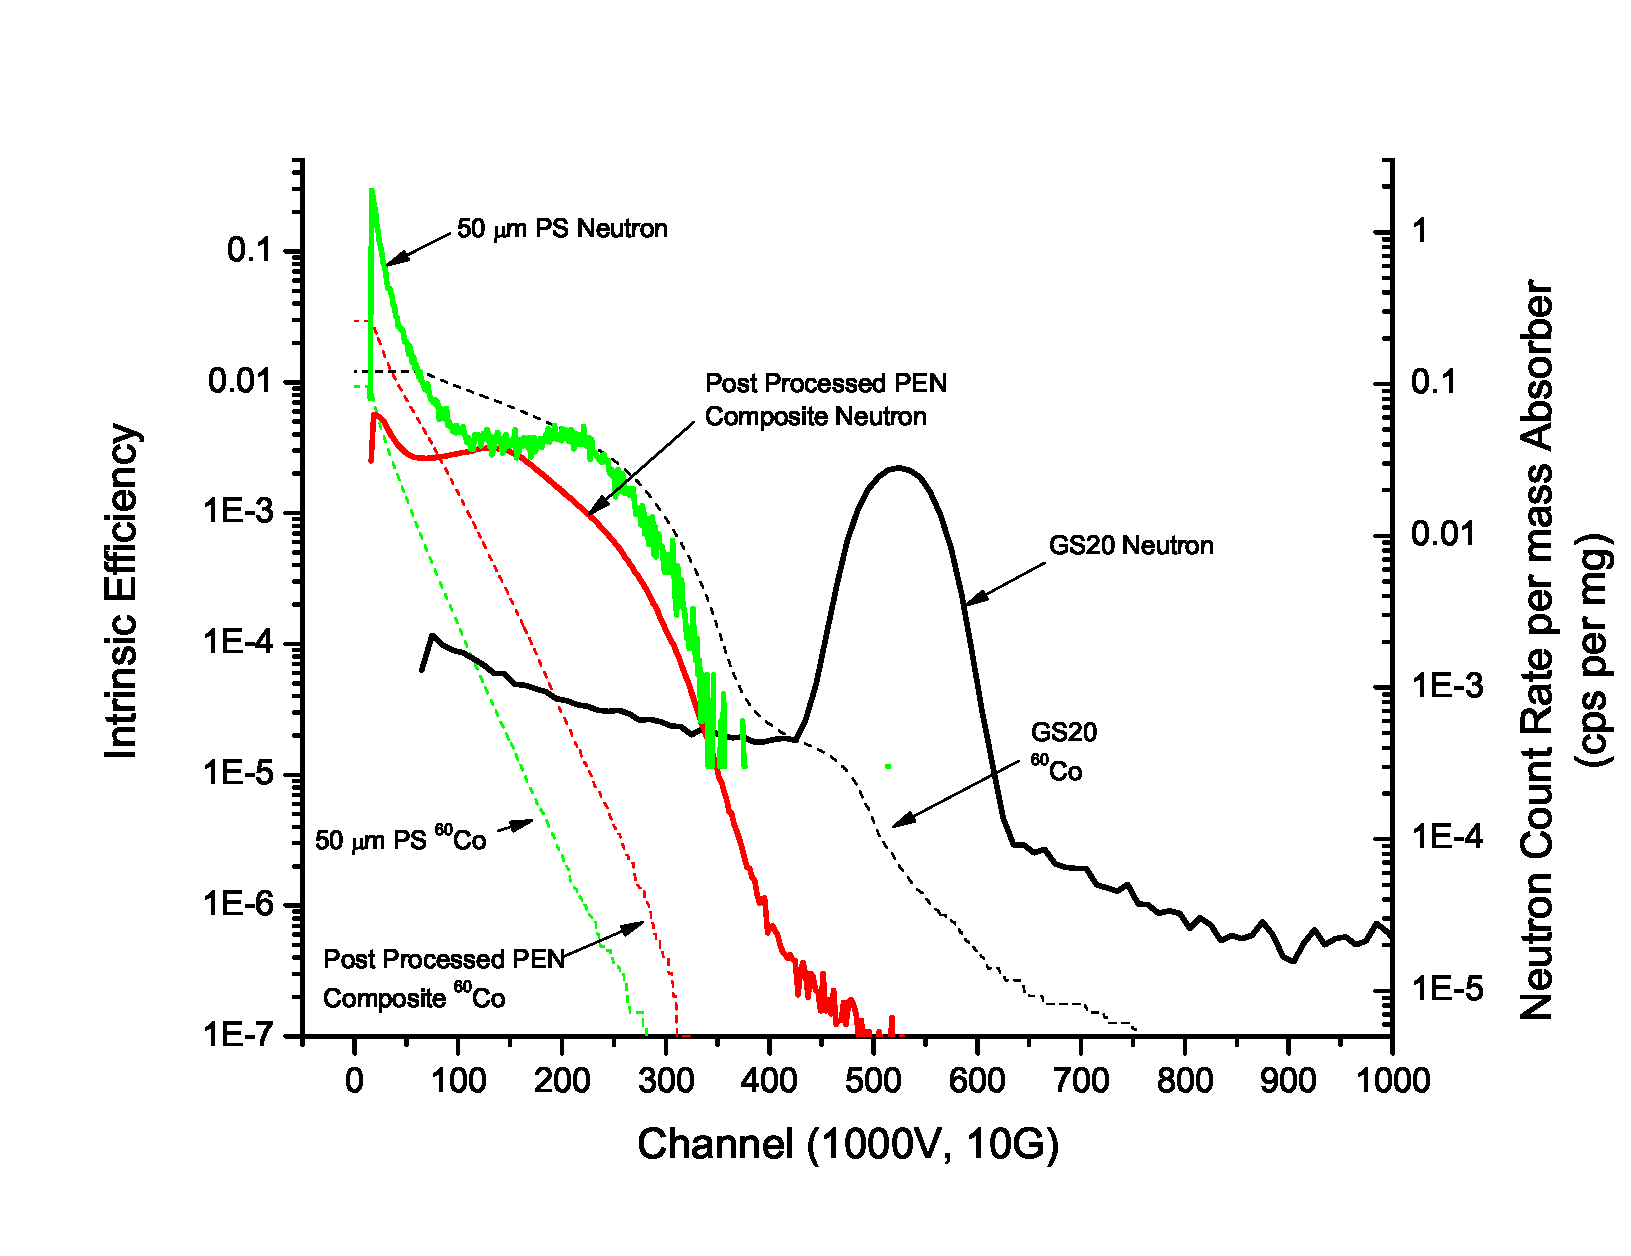
\includegraphics[height=0.6\textheight]{SC_UTDetectors_IntEff_CR}
  \end{figure}
  Pulse height discrimination is equivalent to the energy deposition
\hyperlink{MeasMethods}{\beamerbutton{Measurment Setups and Methods}}
\end{frame}
%%%%%%%%%%%%%%%%%%%%%%%%%%%%%%%%%%%%%%%%%%%%%%%%%%%%%%%%%%%%%%%%%%%%%%%%%%
